%!TEX root = RJwrapper.tex
\title{\pkg{RLumCarlo}: Simulating Cold Light using Monte Carlo Methods}
\author{by Sebastian Kreutzer, Johannes Friedrich, Vasilis
Pagonis, Christian Laag, Ena Rajovic, and Christoph Schmidt}

\maketitle

\abstract{%
The luminescence phenomena of insulators and semiconductors (e.g., natural
minerals such as quartz) have various application domains. For instance,
Earth Sciences and archaeology exploit luminescence as a dating method.
Herein, we present the R package \CRANpkg{RLumCarlo} implementing sets
of luminescence models to be simulated with Monte Carlo (MC) methods. MC
methods make a powerful ally to all kinds of simulation attempts
involving stochastic processes. Luminescence production is such a
stochastic process in the form of charge (electron-hole pairs)
interaction within insulators and semiconductors. To simulate
luminescence-signal curves, we distribute single and independent MC
processes to virtual MC clusters. \CRANpkg{RLumCarlo} comes with a
modularized design and consistent user interface: (1) C++ functions
represent the modeling core and implement models for specific
stimulations modes. (2) R functions give access to combinations of
models and stimulation modes, start the simulation and render terminal
and graphical feedback. The combination of MC clusters supports the
simulation of complex luminescence phenomena.
}

\hypertarget{introduction}{%
\section{Introduction}\label{introduction}}

Light is perhaps the most basic everyday experience. Light emission
that is \emph{not} caused by the heating of a substance is called
luminescence or `cold light'. Various fields exploit this phenomenon.
For instance, Earth Sciences and archaeology determine the timing of
past events (e.g., last sunlight exposure or heating) with a technique
called luminescence dating. Since 2012, the luminescence-dating (or more
general trapped-charge dating) community has gradually adapted R as a
universal tool to analyze, model, and visualize their data. Relevant
related CRAN packages are: \CRANpkg{BayLum} \citep[Bayesian
modeling:][]{Philippe:2019fb, BayLum}, \CRANpkg{Luminescence}
\citep[luminescence- data analysis,][]{Kreutzer:2012ty, Luminescence},
\CRANpkg{numOSL} \citep[luminescence-data
analysis,][]{Peng:2013ws, numOSL}, \CRANpkg{RLumModel}
\citep[luminescence-data modeling,][]{Friedrich:2016kia, RLumModel},
\CRANpkg{RLumShiny} \citep[graphical interface to functions for plotting
and calculation in the framework of luminescence-data analysis,][]{Burow:2016ATL2, RLumShiny}, and \CRANpkg{tgcd} \citep[curve
deconvolution,][]{Peng:2016gc, tgcd}.

\begin{figure}[h]
\begin{center}
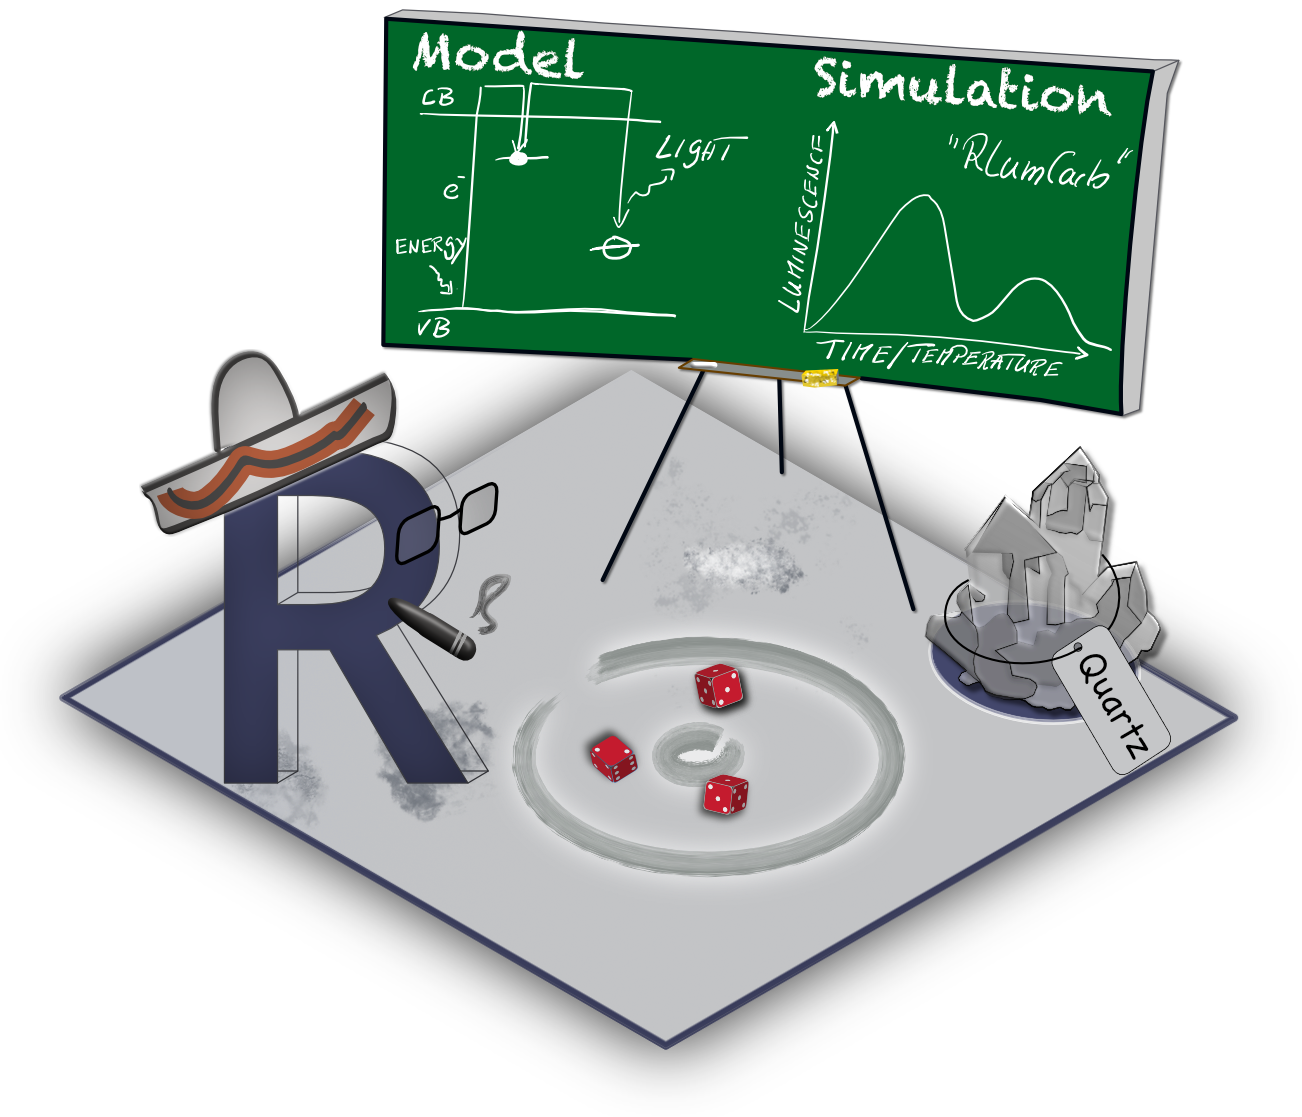
\includegraphics[width=.6\textwidth]{figures/Fig0-1.png}
\caption{\CRANpkg{RLumCarlo} simulates luminescence production in natural minerals such as quartz using Monte Carlo methods. Input is fairly simple (energy-band) models simulating movements of, e.g., electrons in the crystal lattice of quartz. The probability of observing such transitions is a function of energy input in the form of light, heat, or ionizing radiation (e.g., $\beta$- or $\gamma$-radiation). Th output of \CRANpkg{RLumCarlo} is a luminescence curve. This is the light output observed when electrons descend from a higher energy state to a lower energy state emitting part of the energy difference as light.}
\label{fig:Fig0}
\end{center}
\end{figure}
\newpage{}

The luminescence production process is a stochastic process involving
discrete random state transitions of subatomic particles. In the case of
luminescence, this translates to electrons (and holes) moving to
different energy levels, e.g., in the crystal lattice of the natural
mineral quartz. Such processes are ideal for Monte Carlo (MC)
simulations, and their application has a long and propelling history in
physics \citep[cf.][]{Landau:2015vp}. Figure\(~\)\ref{fig:Fig0}
summarizes the purpose of \CRANpkg{RLumCarlo} developed to simulate
luminescence signals in semiconductors and insulators (e.g., quartz)
using MC methods. To that end, \CRANpkg{RLumCarlo} employs simple
(energy-band) models that describe the physical processes in, e.g., the
quartz crystal, to simulate xy-curves (luminescence curves). The
modeling output expresses the evolution of the light production
(luminescence process) over time.

Our contribution, and so \CRANpkg{RLumCarlo}, sits on precedent work by
\citet{Pagonis:2014cs}, \citet{Pagonis:2014gu}, \citet{Pagonis:2019hk},
and \citet{Pagonis:2020bt}. The included collection of energy-band
models for different stimulation modes adapted to MC methods are
valuable for, e.g., studying the impact of model parameters on the
signal-related stochastic uncertainties or statistic effects in tiny,
dosimetric systems. Technically, our approach is closely related to the
simulation of birth-and-death processes \citep[for a review on
birth-and-death process cf.][]{Novozhilov:2006hd}. Each simulation run
describes a Markov process. However, in our case, we allow only a
reduction of an initial number of particles (i.e., only death
processes).

Herein, we will not derive the full theoretical background of the models,
but we will focus on the technical aspects of the package design and the
integration of the MC methods. Such a presentation was beyond the scope
of previous articles \citep[e.g.,][]{Pagonis:2019hk, Pagonis:2020bt},
but it is likely of interest to a broader community.

We structured our contribution as follows. The introduction continues
with a brief paragraph on luminescence and the term `cold light'. After
that, we detail the rationales for our contribution by recalling
conventional modeling approaches in the field. Readers familiar with
these topics may safely skip this part. The subsequent section outlines
the concept and the implementation of \CRANpkg{RLumCarlo}, including
code examples. The remainder addresses (A) the implementation of a
virtual dosimetric system to simulate weak spatial correlation of
dosimetric cluster groups. (B) We outline how \CRANpkg{RLumCarlo} can
simulate more complex models compared to other solutions, with respect
to its strengths and limitations. An outlook outlining the potential to
implement more interactions between models will close our manuscript.

\hypertarget{cold-light-in-a-nutshell}{%
\subsection{`Cold light' in a nutshell}\label{cold-light-in-a-nutshell}}

Light emissions of semiconductors or insulators \emph{after} exposure to
ionizing radiation is a luminescence phenomenon now and then paraphrased
as `cold light'. The term luminescence relates to light production
\emph{not} purely caused by the heating of a substance, a condition
called `incandescence' or black body radiation, but a phenomenon
expressing the inherent capacity of a material (dosimeter) to emit light
(energy) in the ultraviolet to infrared wavelength range
\citep[e.g.,][]{Newton:1957wr, Mahesh_1989fk}. Heat-related luminescence
phenomena of solids have been explored systematically in physics since
the 1930s \citep{Urbach_1930fk} to characterize materials and understand
charge transfers in dosimeters
\citep[e.g.,][]{McKeever_1983ly, Mahesh_1989fk}. The amount of
luminescence, in the context of this manuscript, correlates to the
energy absorbed by a dosimeter during ionizing irradiation. The closest
analogy to a dosimeter is a battery that can be charged by, e.g.,
\(\gamma\)-radiation and discharges while emitting light. Natural
minerals such as quartz or feldspar are dosimeters. Defects and
impurities in their crystal lattice can trap charges (electrons or
holes) in metastable states between valence and conduction band. The
time an electron spends in such a state can vary from a fraction of a
second to millions of years, depending on the crystal lattice
configuration and the environmental conditions. The amount of
(potential) energy held by an electron in such a center is approximately
the energy difference between the valence band and the energy level of
the center. A transition of the electron to a lower energy state may
lead to a photon emission of the form
\(E_{photon} = \hbar\omega_{nm} = E_{n} - E_{m}\)\footnote{$\hbar$ (eV$~$s): Planck constant divided by $2\pi$; $\omega$ (radians per s): frequency; $E_{n}$ (eV): higher energy state; $E_{m}$ (eV): lower energy state}.
Energy input (`stimulation') can move the electron out of the defect and
eventually it recombines with a hole trapped at another defect
(`recombination centre'). Types of stimulation methods relevant for our
contribution are heat (thermally stimulated luminescence, TL), visible
light (optically stimulated luminescence, OSL), and infrared light
(infrared stimulated luminescence, IRSL).

Luminescence phenomena have versatile use in the fields of personal,
medical, and accidental dosimetry \citep[e.g.,][]{Yukihara_2011zr}. As
aforementioned, in Earth Sciences and archaeology, the luminescence of
natural minerals gained considerable attractiveness as a dating method
(luminescence dating). First attempts exploiting luminescence signals as
a chronological tool reach back to the 1950s
\citep{Daniels:1953hw, Houtermans:1957vu, Grogler_1958fk}. Nevertheless,
it needed a few decades more before the method took off and became today
one of the most frequently used dating methods on sediments for the last
250,000 years and beyond
\citep[e.g.,][]{Aitken_1985dq, Aitken_1998eu, Bateman:2019wy}.

\hypertarget{towards-monte-carlo-simulations}{%
\section{Towards Monte Carlo
simulations}\label{towards-monte-carlo-simulations}}

To explain luminescence production, \citet{Johnson:1939iy} and
\citet{Randall:1945je} introduced the first basic energy-band models. Today,
most of the commonly accepted luminescence models use series of more or
less complicated systems of differential equations \citep[for an
overview, see][]{Chen:1997dr, Botter-Jensen_2003uq, Chen_2011ij}
employing energy-band models. Those models provide a proper
phenomenological match with measured data for various experimental
designs by simulating electronic transitions. 'Conventional' energy-band
models available to simulate luminescence production are developed as a
set of nonlinear differential equations. This brings some limitations:

\begin{enumerate}
\def\labelenumi{\arabic{enumi}.}
\tightlist
\item
  The models become complex easily and cannot be solved analytically.
\item
  If numerical methods are used, some equations are numerically
  unstable, which may lead to wrong simulation results.
\item
  A convenient assumption in many of such models is a great abundance of
  spatially uniformly distributed traps and recombination centers.
  However, this is not always the most prudent assumption. A spatial
  correlation and cluster formation of centers may exist for various
  reasons \citep[cf.][]{Mandowski:1992ke, Chen_2011ij, Horowitz:2017eo}.
\item
  Deterministic models do not consider stochastic uncertainties and
  simulated curves are `noise free'. These limits subsequent analyses for
  materials where such uncertainties would matter due to the low,
  finite, number of charge carriers, and in these scenarios, simulation
  results are used as reference data to test statistical models used for
  luminescence data analysis in general.
\end{enumerate}

Modeling code for simulating luminescence production was often written
with the tools at hand, e.g., \emph{Mathematica}
\citep[e.g.,][]{Pagonis_2006ve}, which has led to a fragmentation of
incompatible solutions. In 2016, \citet{Friedrich:2016kia} introduced
\CRANpkg{RLumModel} \citep{RLumModel}, pooling available kinetic (non-MC)
models available for the luminescence production in quartz. A tantamount
suite of R code was presented simultaneously by \citet{Peng:2016jg}. We
will compare results from \CRANpkg{RLumModel} and \CRANpkg{RLumCarlo} at
the end of this manuscript.

MC simulations offer an alternative and are indispensable if the
simulation of defect clusters in combination with the analysis of
stochastic uncertainties is desired. Usually, the underlying models are
very simple, but can be combined to describe complex systems. Important
early work simulating TL using MC methods goes back to
\citet{Mandowski:1992ke} and \citet{Kulkarni:1994dr}.
\citet{Mandowski:1992ke} tried to overcome the prerequisite of a large
number of sample carriers, and \citet{Kulkarni:1994dr} investigated MC
methods to overcome very long calculation times encountered for
numerical calculations in particular scenarios. \citet{Kulkarni:1994dr}
(p.~103) also reported a ``statistical fluctuation'' (noise like
scatter) caused by the MC simulations but considered this more as a
disadvantage. Later, \citet{Pagonis:2020bt} explicitly exploited this as
a feature, similar to birth-and-death processes and their related random
uncertainties, to investigate specifically the stochastic uncertainties.

Before we start to detail \CRANpkg{RLumCarlo}, a preceding note of
caution: Any attempt to answer the question of whether a particular
model may better explain the one or the other effect measured in
luminescence studies would open Pandora's box
\citep[e.g.,][]{Horowitz:2017eo}. Consequently, we will not engage in
such a discussion. What we have implemented so far in
\CRANpkg{RLumCarlo} can be modified and exchanged. However, the
underlying design concept remains applicable.

\hypertarget{the-concept-of}{%
\section{\texorpdfstring{The concept of
\CRANpkg{RLumCarlo}}{The concept of }}\label{the-concept-of}}

\CRANpkg{RLumCarlo} implements energy-band models in a modular approach.
Each model can simulate only an isolated effect (e.g., a single curve,
see below), but the package design allows various combinations, e.g., in
the form of clusters. Hence, \CRANpkg{RLumCarlo} can evolve beyond a
specific mathematical model through a combination of simple models.

To that end, \CRANpkg{RLumCarlo} differs fundamentally from
\CRANpkg{RLumModel}, where the collected models allow the simulation of
complex phenomena and even entire measurement sequences
\citep{Friedrich:2016kia} but are self-contained by design. In other
words, simulations cannot evolve beyond a specific mathematical model
selected by the user. In \CRANpkg{RLumCarlo}, the implemented energy-band
models can simulate only isolated effects (e.g., a single curve, see
below), but the package design allows a combination in the form of
clusters. Throughout the text, we will use the word `clusters' to (1)
ascribe virtual units used in the MC simulation to run independent
random processes (henceforth MC clusters) and (2) to define groups of
defects (defect clusters) e.g., defined by their spatial distance. Only
the latter carry a physical meaning.

\hypertarget{implemented-energy-band-models}{%
\subsection{Implemented energy-band
models}\label{implemented-energy-band-models}}

\begin{Schunk}
\begin{figure}

{\centering 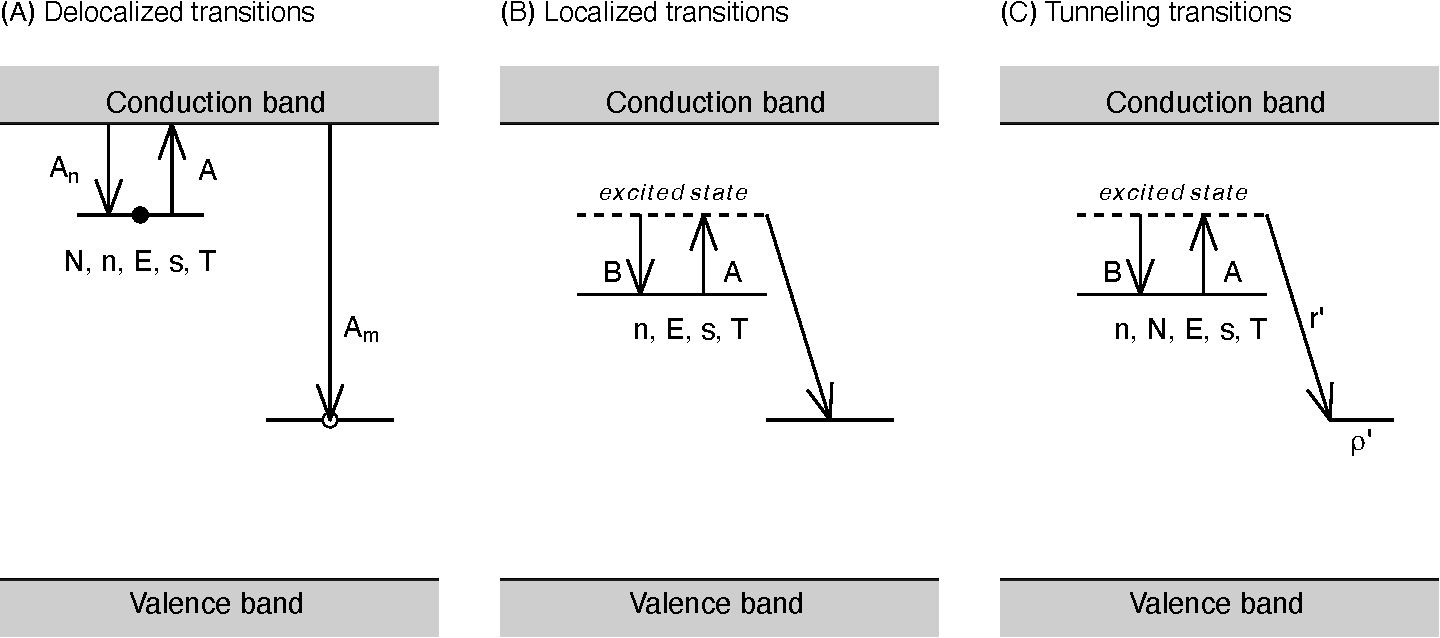
\includegraphics[width=140mm]{figures/Fig1-1} 

}

\caption{Energy-band model representation of the models implemented in \CRANpkg{RLumCarlo}. Letters represent physical model parameters, and arrows indicate allowed transitions. (A) Delocalized transition: the model consists of one single trap and one recombination center. Transition processes involve the conduction band. (B) Localized transition: the model consists of two sub-conduction band energy levels. Charge transitions do not involve the conduction band but take place locally with a constant recombination rate. (C) Tunneling transition: The model consists of one trap and one recombination center. Transitions take place from the excited state into the recombination center without involving the conduction band, and the recombination rate depends on the distance between electrons and holes. All symbols are detailed in the package manual, the package vignette, and the main text. Side note: For the creation of the plots we used \CRANpkg{scales} and \CRANpkg{ggplot2} (\url{https://github.com/JohannesFriedrich/EnergyBandModels}).}\label{fig:Fig1}
\end{figure}
\end{Schunk}

To date, \CRANpkg{RLumCarlo} ships three simple energy-band models
(Figure\(~\) \ref{fig:Fig1}) to simulate luminescence production using
(A) delocalized transitions, (B) localized transitions, and (C) excited
state tunneling transitions. The models are distinguished by the
allowed routes of electrons involved in the luminescence process from
one energy state to another. Only the first model (Figure\(~\)
\ref{fig:Fig1}A) involves the conduction band, while the models in
Figures\(~\)\ref{fig:Fig1}B and C limit the allowed electron pathways to
energy levels below the conduction band.

While the parameters differ from model to model and depend on the
stimulation mode (heat or light, continuous or ramped), key entities
remain alike across the models, such as the trap depth (the energy
difference of the electron state from the conduction band) \(E\) (eV),
the attempt to escape frequency of an electron from the trap (short:
frequency factor) \(s\) (s\(^{-1}\)), the temperature \(T\) (K), and the
trapped concentration of electrons \(n\) (cm\(^{-3}\)) in the trap.
\(N\) (models A and B) is the total number of available electrons in
cm\(^{-3}\) and \(\rho'\) is the dimensionless density of recombination
centers \citep[model C,][]{Huntley:2006gs}. The symbols \(A_n\), \(A_m\),
and \(A\) (model A), \(B\) and \(A\) (model B), and \(B\), \(A\), and
\(r'\) (model C) plotted next to the arrows in Figure\(~\)
\ref{fig:Fig1} parametrize, simply put, the rates of the electronic
transitions.

\begin{figure}[h]
\begin{center}
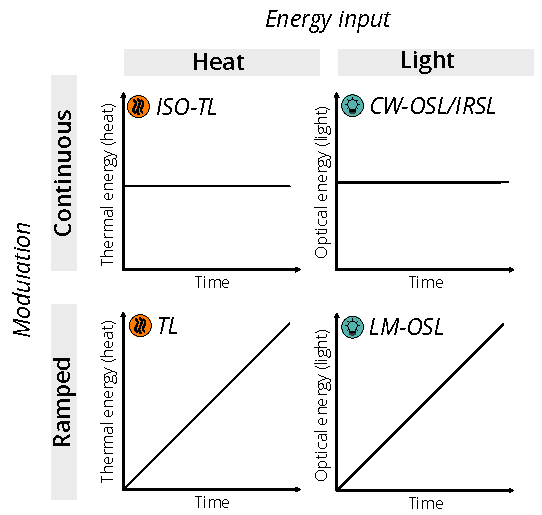
\includegraphics[width=.5\textwidth]{figures/Fig2-1.pdf}
\caption{Stimulation modes in \CRANpkg{RLumCarlo} applicable to the models. ISO-TL: isothermal TL, i.e., constant stimulation temperature over time. TL: thermal luminescence, i.e., temperature ramps (approximately linearly) over time. CW-OSL/IRSL: continuous wave optically stimulated luminescence respectively infrared stimulated luminescence, constant optical stimulation over time. LM-OSL: linearly modulated optically stimulated luminescence, i.e., linearly ramped optical stimulation over time.}
\label{fig:Fig2}
\end{center}
\end{figure}

The conditions of the simulations are defined through these parameters,
with \(n\) being the crucial number. Once the electrons have all
recombined, the simulation may still continue, but the luminescence
signal is zero. As we will detail below, the essential point of the MC
simulation, from the physical point of view, is that these
concentrations become dimensionless, absolute numbers in a finite
system.

Each model supports up to four different stimulation modes (Figure\(~\)
\ref{fig:Fig2}), i.e., the type of energy input (light or heat) and its
modulation (continuous or ramped).

As an example, we will detail the mathematical background and its
implementation for delocalized transitions below. For all other models,
we may refer to the cited literature as well as the package manual.

\hypertarget{conceptional-overview-of-the-implementation}{%
\subsection{Conceptional overview of the
implementation}\label{conceptional-overview-of-the-implementation}}

The basic implementation of the MC processes as a software algorithm
consists of two nested loops. The outer loop iterates over a time
\(0<t\leqslant t_{max}\) with \(t \in \mathbb{R} > 0\). The inner part
loops over particles \(0<j\leqslant n\) with \(n \in \mathbb{Z}\). The
model tests a random number, newly sampled with replacement in each run,
against a threshold \(P\). If the sampled random number is smaller than
\(P\), the absolute number of particles is reduced by one. The code
below shows the basic algorithm outlined above for the radioactive
decay, which we have chosen because it can be found in standard
textbooks \citep[e.g.,][]{Landau:2015vp}. Below we used R code for
illustrative reasons, while the package implementation is written in
C++.

\begin{Schunk}
\begin{Sinput}
n <- 1000
t <- 1:100
P <- 0.2
remaining <- numeric(length(t))

for (t in t) {
  for (j in 1:n) {
    if (runif(1) < P && n > 0)
      n <- n - 1
    
  }
  
  if (n > 0)
    remaining[t] <- n
  
}
\end{Sinput}
\end{Schunk}

For example, the algorithm starts with 1,000 particles. In time instant
\(t_1\), the random number was smaller for two particles \(j_6\) and
\(j_{576}\). Hence, in time instant \(t_2\), the inner loop iterates only
over \(j = \{1,2,...,998\}\) particles. The absolute number of remaining
particles for each \(t\) is stored in a vector of length
\(t_{max}/\Delta t\). This vector is the observed signal curve (in the
case of luminescence, the righthand side graph on the green board in
Figure\(~\) \ref{fig:Fig0}).

\hypertarget{implementation-example-for-the-otor-model}{%
\subsection{Implementation example for the OTOR
model}\label{implementation-example-for-the-otor-model}}

The implementation for luminescence production in \CRANpkg{RLumCarlo} is
very similar. To exemplify the adaptation of the models to be run as an
MC simulation, we have selected the one-trap one-recombination center
(OTOR) model \citep[based on][]{Halperin:1960gr} for TL. Our description
below follows \citet{Pagonis:2014cs}.

The OTOR model for TL can be expressed with the following set of
differential equations:

\begin{equation}
\frac{dn}{dt} = -ns~exp\big(-\frac{E}{k_{B}T}\big) + n_c(N-n)A_{n}
\end{equation}

\begin{equation}
\frac{dn_{c}}{dt} = -\frac{dn}{dt} - n_{c}mA_{m}
\end{equation}

\begin{equation}
I_{TL}(t) = -\frac{dm}{dt}= n_{c}mA_{m}.
\end{equation}

Beyond already mentioned symbols, we used in the equations \(I_{TL}\),
the time-dependent intensity, and \(n_c\) (cm\(^{-3}\)), the current
concentration of electrons in the conduction band. The concentration of
recombination centers is represented by \(m\) (cm\(^{-3}\)), where for
reasons of charge neutrality \(m = n + n_{c}\). \(A_{n}\) and \(A_{m}\)
(both in cm\(^{3}\,\)s\(^{-1}\)) are the capture coefficients for traps
and recombinations centers, respectively. \(k_{B}\) (eV\(\,\)K\(^{-1}\))
is the Boltzmann constant and \(T\) (K), the absolute temperature.

By assuming quasi-static equilibrium conditions \citep{Chen_2011ij}
\begin{equation}
\Big|\frac{dn_{c}}{dt}\Big| \ll \Big|\frac{dn}{dt}\Big|,\Big|\frac{dm}{dt}\Big|~~;~~ n_{c} \ll n, ~~ 
n \simeq m, 
\end{equation}

the resulting TL intensity becomes the general one trap equation, GOT:

\begin{equation}
I_{TL}(t) = -\frac{dn}{dt} = s~exp(-\frac{E}{k_{B}T})~\frac{A_{m}n^{2}}{(N-n)A_{n} + nA_{m}}.
\end{equation}

\begin{equation}
T = T_{0} + \beta \times t,
\end{equation}

\noindent{}with \(T\) (K) and \(T_{0}\) (K) being temperatures, \(\beta\)
(K\(\,\)s\(^{-1}\)) the (heating) rate, and \(t\) (s) the simulation
time. \(p(t) = s~exp(-\frac{E}{k_{B}T})\) is the rate of thermal
excitation, and \(R = \frac{A_{n}}{A_{m}}\) is the dimensionless
retrapping ratio. The translation into a finite system with a discrete
distribution of charge carriers
\citep[cf.][]{Mandowski:1991ha, Mandowski:1994fi}, can be expressed
through

\begin{equation}
\chi n,\chi N \rightarrow{} \bar{n}, \bar{N},
\end{equation}

\noindent{}and the differential equation becomes a difference equation:

\begin{equation}
I_{TL}(t) = -\frac{1}{\beta}\frac{\Delta \bar{n}}{\Delta t} = p(t) \frac{\bar{n}^2}{\bar{N}R + \bar{n}(1-R)}. 
\end{equation}

\noindent{}\(\chi\) (cm\(^3\)) is a constant, \(\bar{n},\bar{N} \in \mathbb{Z}\),
and \(\Delta t = 1\,\)s is an appropriate time interval. \(R\) is the
dimensionless re-trapping ratio in the finite system. To simulate the
luminescence process, the related Markov process renders similar to the
theory of birth-and-death processes \citep[e.g.,][]{Novozhilov:2006hd},
where the population (here of electrons) decreases over continuous time
with the probability to observe a transition within \(\Delta t\) being
\(P = \mu_{\bar{n}} \Delta t\) (here \(\mu_{\bar{n}}\) is the
``death-rate'' in s\(^{-1}\)) until the population is depleted. The
so-called `brute force' approach \citep[e.g.,][]{Landau:2015vp} tests
the population of electrons (\(\bar{n}\)) per integer time
step sequentially by comparing it against a random number sampled with replacement
from a continuous distribution \(r \sim \mathcal{U}(0,1)\) against the
conditional probability \(P\) for an electron to get evicted from the
trap. In our case, \(P\) is calculated as follows:

\begin{equation}
p(t) \times \delta t \times \frac{n}{\bar{N}R + \bar{n}(1-R)}.
\end{equation}

The factor \(\delta t\) allows values of \(\Delta t \neq 1\) while
ensuring that \(P \ll 1\). \(p(t)\) depends on the stimulation mode and
the chosen model. For TL (functions named
\texttt{run\_MC\_TL\_\textless{}model\textgreater{}()}) and isothermal
TL (functions named
\texttt{run\_MC\_ISO\_\textless{}model\textgreater{}()}) applying the
localized or delocalized model \(p(t)\) becomes:

\begin{equation}
p(t) = s~exp(-\frac{E}{k_{B}T}),
\end{equation}

\noindent{}and for TL, from tunneling transitions it reads:

\begin{equation}
p(t) = s~exp(-\frac{E}{k_{B}T})~exp(-\rho'^{-1/3}r'),
\end{equation}

\noindent{}with \(\rho'\) being the dimensionless concentration of recombination
centers, and \(r'\) being the dimensionless tunneling radius
\citep{Huntley:2006gs}. The basic structure in \CRANpkg{RLumCarlo} is,
however, identical, except for the models based on excited-state
tunneling. Here, an additional outer loop iterates over the
dimensionless tunneling radius \(0 \leqslant r' \leqslant 2\)
\citep{Huntley:2006gs}.

\hypertarget{the-package-design}{%
\subsection{The package design}\label{the-package-design}}

\begin{figure}[h]
\begin{center}
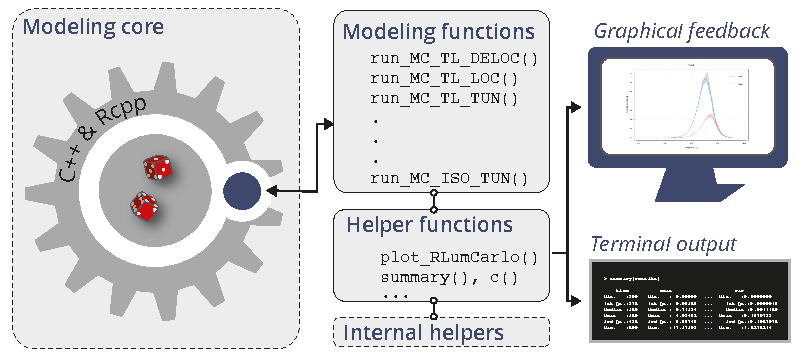
\includegraphics[width=.8\textwidth]{figures/Fig3-1.pdf}
\caption{The conceptional design of \CRANpkg{RLumCarlo}. User interaction is realized via exported R functions, one function for each model and stimulation type. For the MC runs, we use C++ functions interfaced via \CRANpkg{Rcpp}. Helper functions support 
graphical and terminal feedback.}
\label{fig:Fig3}
\end{center}
\end{figure}

In Figure\(~\) \ref{fig:Fig3}, we outline the basic layout of
\CRANpkg{RLumCarlo}. Two design decisions stand out: (1) Each
stimulation mode/energy-band model combination has its own exported R
function commencing with the prefix \texttt{run\_MC}. (2) These
functions interface one C++ function, each via \CRANpkg{Rcpp}
\citep{Rcpp} (for an overview, see the vignette of \CRANpkg{RLumCarlo}).
The R functions provide a convenient user interface, and the C++
functions constitute the workhorse, as shown in the modeling core
(Figure\(~\) \ref{fig:Fig3}). While the apparent reason for using C++
was speed, the implementation could have been programmed more concisely,
i.e., completely in C++ instead of interfacing C++ with R. However, we
wanted to allow code inspection by non-specialists from our field, who
may wish to implement other models alike. We found that the separation
of the user interface (in R) from the modeling core (in C++) aligns
best with our premise of simplicity and flexibility.

As indicated above in the example implementation algorithm, each
simulation run \citep[ used the term `particle
tracking']{Kulkarni:1994dr} starts with \(n > 1\) and ends at
\(t_{max}\), while \(I(t) = 0\) for \(n = 0\). In reality, one has to
execute several simulation runs separately (henceforth `MC clusters', to
be distinguished from defect clusters), either to reduce the statistical
fluctuation or to estimate the stochastic error \citep{Kulkarni:1994dr}.
\CRANpkg{RLumCarlo} runs the simulations in virtual MC clusters on
single or multicore systems using \CRANpkg{parallel} \citep{parallel},
\CRANpkg{doParallel} \citep{doParallel}, and \CRANpkg{foreach}
\citep{foreach} supported by helper functions (Figure\(~\)
\ref{fig:Fig3}), to summarize results and to provide S3-class based
graphical output.

\hypertarget{simple-illustrative-examples}{%
\section{Simple illustrative
examples}\label{simple-illustrative-examples}}

\begin{Schunk}
\begin{figure}

{\centering 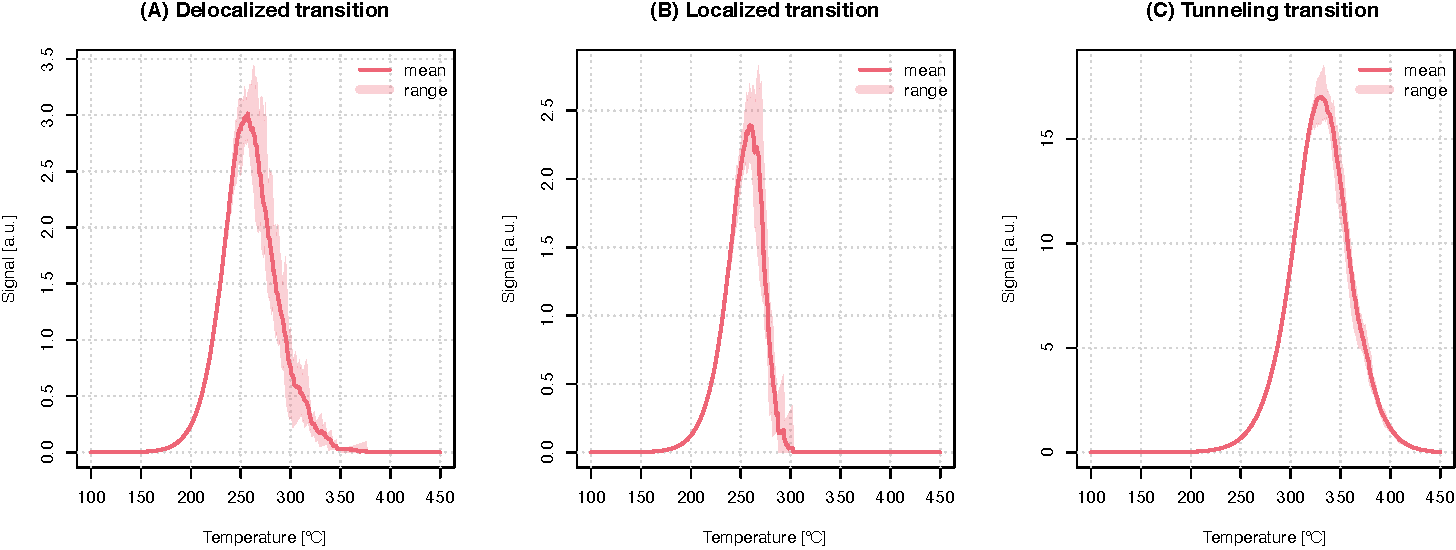
\includegraphics[width=140mm]{figures/Fig4-1} 

}

\caption{Exemplary comparison of TL signals simulated for all three \CRANpkg{RLumCarlo} models: (A) delocalized (DELOC), (B) localized (LOC), and (C) tunneling (TUN). General physical parameters, such as $E$ (1.45$\,$eV), $s$ ($3.5\times10^{12}\,$s$^{-1}$), and the stimulation temperature (100--450$\,^{\circ}$C) were kept constant for all models.}\label{fig:Fig4}
\end{figure}
\end{Schunk}

Simulations start with a call of the respective function, e.g., for
\texttt{TL} using the \texttt{DELOC} model \texttt{run\_MC\_TL\_DELOC()}
or \texttt{run\_MC\_TL\_LOC()} for the \texttt{LOC} model, respectively
(see Figures\(~\)\ref{fig:Fig1}A-B).

\begin{Schunk}
\begin{Sinput}
results <- run_MC_TL_DELOC(
 s = 3.5e12,
 E = 1.45,
 clusters = 10,
 n_filled = 200,
 R = 1,
 times = 100:450)
\end{Sinput}
\end{Schunk}

The function parameter names follow the terminology used for the
mathematical expression of the models as closely as possible. For
example, \texttt{E} and \texttt{s} are \(E\) (trap depth in eV) and
\(s\) (frequency factor in s\(^{-1}\)). \texttt{R} (\(R\) in Figure\(~\)
\ref{fig:Fig2}) is the so-called re-trapping ratio, expressing the
chance an electron of \emph{not} passing into the conduction band, and
\texttt{n\_filled} is \(\bar{n}\), the number of electrons at the
beginning of the simulation. The duration of the simulation on the time
domain (which is not the duration of the computation) is set by
\texttt{times}. The parameter \texttt{clusters} sets the number of MC
clusters, i.e., the number of Markov chains. High numbers in
\texttt{clusters} increase the confidence in the simulation output at
the cost of more computation time.

The output can be passed to a dedicated plot function
(\texttt{plot\_RLumCarlo()}). The function supports a couple of standard
plot arguments, such as \texttt{main} for the title of the plot, which
is passed down to \texttt{graphics::plot.default()} via \texttt{...}
(type \texttt{?dots} in the R terminal).

\begin{Schunk}
\begin{Sinput}
plot_RLumCarlo(
  object = results,
  legend = TRUE, 
  main = "(A) Delocalized transition")
\end{Sinput}
\end{Schunk}

\begin{Schunk}
\begin{figure}

{\centering 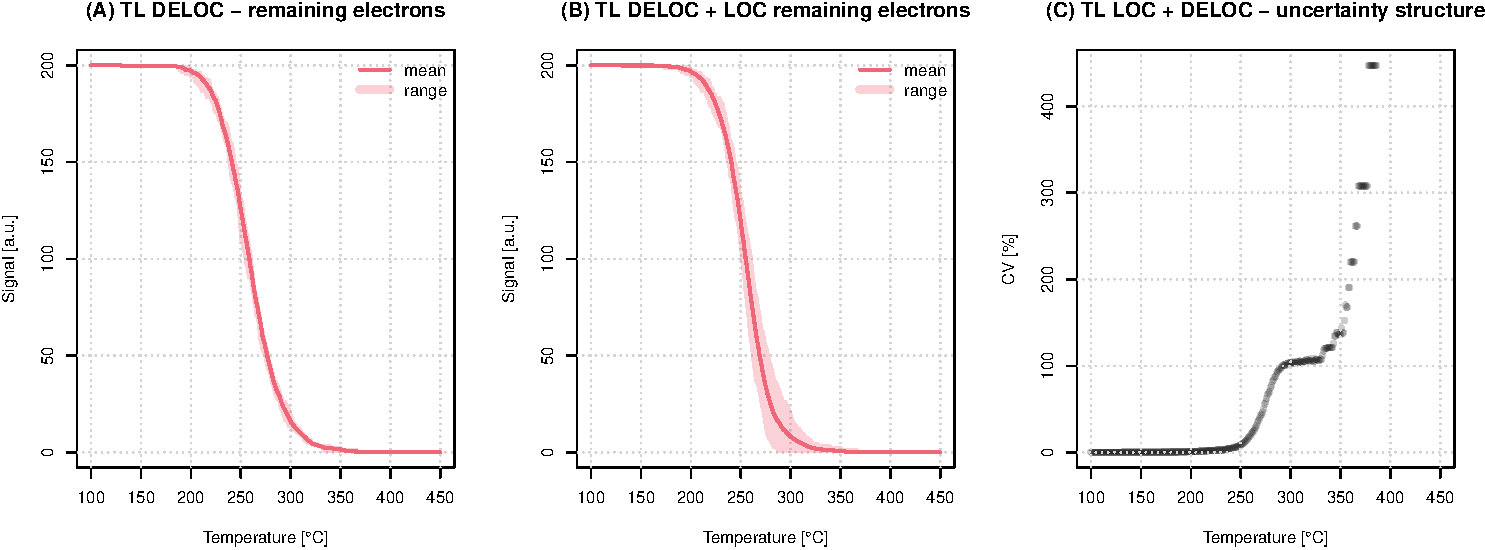
\includegraphics[width=140mm]{figures/Fig5-1} 

}

\caption{(A) Plot of the remaining electrons for the TL process using the delocalized transition model for which we show the luminescence signal in Figure~\ref{fig:Fig4}A. (B) Plot of remaining electrons for two models combined in one system. (C) Stochastic uncertainty structure from (B).}\label{fig:Fig5}
\end{figure}
\end{Schunk}

The parameter \texttt{n\_filled} can be a vector enabling different
starting conditions for each MC cluster. Figure\(~\)\ref{fig:Fig4}A
shows the graphical output for delocalized transitions along with the
simulation results for \texttt{TL} stimulation using localized
(Figure\(~\) \ref{fig:Fig4}B) and tunneling transitions (Figure\(~\)
\ref{fig:Fig4}C). The output is an object of class
\texttt{RLumCarlo\_Model\_Output}, which is a \texttt{list} comprising a
multi-dimensional \texttt{array} (one slice per MC cluster) with the
resulting luminescence signal and a \texttt{numeric} vector for the
stimulation time.

Currently we provide S3-generics for \texttt{summary()} and
\texttt{c()}. The first one is also used internally by
\texttt{plot\_RLumCarlo()} to melt the array into a \texttt{data.frame}
before plotting. The plot output adapts to the used stimulation mode
provided via an attribute with each output object.

A straightforward application for this kind of simulation is the study
of the impact of physical parameters on the luminescence signal output
and the estimation of the stochastic uncertainties, which cannot be
achieved with the deterministic approach of differential equations.

We provide more, always up-to-date examples with the package vignette,
where we also compiled a table with meaningful physical parameter ranges
for each model.

\hypertarget{advanced-examples-and-further-considerations}{%
\subsection{Advanced examples and further
considerations}\label{advanced-examples-and-further-considerations}}

The examples so far presented may not appear very sophisticated, and
still, they allow insight that goes beyond a simple educational purpose
of simulating luminescence based on phenomenological models.
\citet{Pagonis:2020bt}, who used a preliminary version of
\CRANpkg{RLumCarlo}, addressed in detail the stochastic uncertainties of
TL and OSL models. These uncertainties come into play in nano-dosimetric
materials with a small number of defect clusters where the
``finite-size'' \citep{Mandowski:1991ha} of the system starts to matter
in terms of a presumed spatial correlation of defect cluster groups. To
some extent, this should also be true for systems exposed to high-energy
radiation causing defect clusters
\citep[e.g.,][]{Mandowski:1991ha, Mandowski:1992ke}. Previously in this
paper, we have used the term `MC clusters'. For a start, in
\CRANpkg{RLumCarlo}, `MC clusters' entail independent and continuous
Monte Carlo Markov chains employed to simulate luminescence production,
starting with a particular number of electrons in the system. Whether
the processes are run in parallel or sequentially has no impact on the
outcome, except for computation speed. In other words, `MC clusters'
carry no meaning regarding the underlying physics. However, as mentioned
above, `MC clusters` from different models (with the same stimulation
mode) can be concatenated (see Figure\(~\) \ref{fig:Fig5}B-C) to
simulate defect clusters (also, dosimetric clusters), to which we can
attribute physical meaning.

\hypertarget{spatial-correlation}{%
\subsubsection{Spatial correlation}\label{spatial-correlation}}

To simulate a three-dimensional (dosimetric) system, we can add meaning
to MC clusters by reinterpreting them as dosimetric clusters. From the
modeling perspective, nothing changes, but MC clusters gain a
connotation of having a physical meaning.

Figure\(~\)\ref{fig:Fig6}A illustrates the situation of model
combinations transferred into a virtual, three-dimen-sional dosimetric
system. Since all defect clusters are distributed evenly over the
system, the distance to each neighboring point is identical, and it is
a constant rather than a variable. In other words, the spatial distance
between neighboring points does not matter and is of no relevance for
the simulation but here chosen for illustrative reasons only.
Figure\(~\)\ref{fig:Fig6}B represents a situation that takes one step
further. Here, the points are randomly distributed over the system, and
points form groups (defect cluster groups). Additionally,
\CRANpkg{RLumCarlo} supports the mixing of models for the same stimulation
mode as in Figure\(~\) \ref{fig:Fig6}A (not shown here). The driving
idea of the implementation is the assumption of an individual spatial
ordering of defects in a, e.g., quartz crystal to which the luminescence
production process might be assigned based on models mentioned above.

Such a system can be created in \CRANpkg{RLumCarlo} via
\texttt{create\_ClusterSystem()}. The function distributes points
randomly with their coordinates:

\begin{equation}
x_1,y_1,z_1,...,x_k,y_k,z_k \sim \mathcal{U}(0,1)~\mathtt{|}~k \in \mathbb{Z}.
\end{equation}

\begin{figure}[h]
\begin{center}
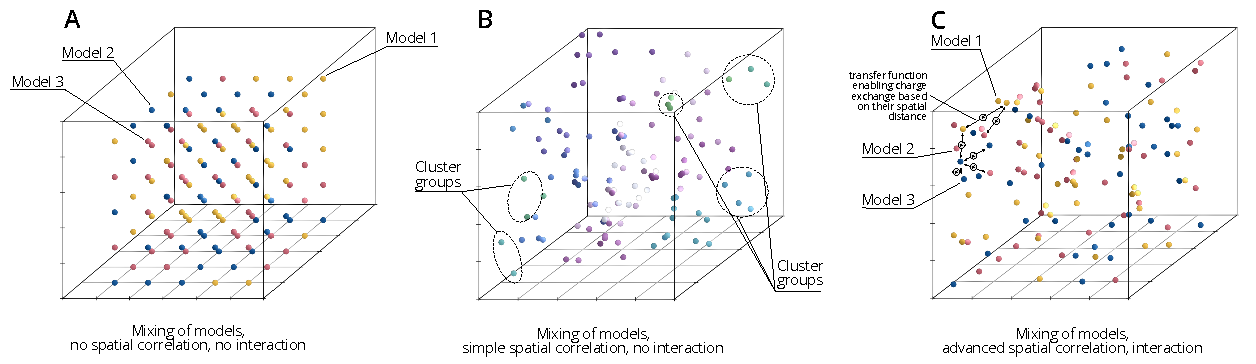
\includegraphics[width=1\textwidth]{figures/Fig6-1.pdf}
\caption{A dosimetric system with three possible approaches of cluster 
correlation and interaction. (A) Models can be mixed, but no spatial correlation 
is realized, and no interaction possible. This is the basic mode in \CRANpkg{RLumCarlo}. 
(B) Clusters are grouped by their Euclidean distance, and models can be mixed. Electrons
are distributed according to the spatial distance of clusters and also models
can be mixed (not shown in the figure). The advanced mode in \CRANpkg{RLumCarlo}. 
(C) Clusters can interact with each other and even exchange electrons. This last 
stage is subject to future developments of \CRANpkg{RLumCarlo}.}
\label{fig:Fig6}
\end{center}
\end{figure}

Then, the Euclidean distance between the points is determined with
\texttt{stats:dist()}, which is used by \texttt{stats:hclust()} to group
the defect clusters (\(\Xi\)). To avoid too many small groups, we then
cut the cluster tree using \texttt{stats:cutree()}, with the outcome
shown in Figure\(~\) \ref{fig:Fig6}B. The selection of
\texttt{stats:hclust()} and \texttt{stats:cutree()} for defining the
clusters is somewhat arbitrary and might be refined in the future.
Therefore, more research, supported by measurements, is needed.

Now, any function from \CRANpkg{RLumCarlo} can be used, and the output of
\texttt{create\_ClusterSystem()} is taken as input for the argument
\texttt{clusters}. For example:

\begin{Schunk}
\begin{Sinput}
run_MC_TL_LOC(s = 3.5e12, E = 1.45, n_filled = 1000,
  clusters = create_ClusterSystem(100))
\end{Sinput}
\end{Schunk}

\noindent{}creates a system with 100 randomly distributed defect clusters. If the
simulation is run in such a mode, the meaning of \texttt{n\_filled}
changes. Previously, it defined the number of electrons in each cluster
(\(\bar{n}_{cl_i}\)). However, now the same parameter defines the total
number of electrons in the entire system. The number of electrons in the
\(i\)th cluster (\(\bar{n}_{cl_i}\)) is then an integer fraction of
electrons available in each cluster group
(\(\bar{n}_{\Xi_{i}} = \mathtt{n\_filled}/ N_{\Xi}\), with \(N_{\Xi}\)
the total number of cluster groups). The more clusters are in one group,
the less electrons are available per cluster in the group and vice
versa. While this is a very simple approach, it allows us to simulate
basic spatial correlation. Figure\(~\)\ref{fig:Fig6}C drafts a better
way of mimicking spatial interaction of clusters, which is, however, not
yet part of \CRANpkg{RLumCarlo}. While it would be, based on the
designed system, easy from the programming perspective, the needed
equations to describe to exchange electrons are yet to be developed.

\hypertarget{comparison-to}{%
\subsubsection{\texorpdfstring{Comparison to
\CRANpkg{RLumModel}}{Comparison to }}\label{comparison-to}}

In the remainder, we want to compare simulation results from
\CRANpkg{RLumCarlo}, with other types of solutions, such as
\CRANpkg{RLumModel} which uses coupled differential equations to
simulate luminescence production. \CRANpkg{RLumModel} was selected since
it was developed by some of the authors of this contribution. However,
in theory, simple scripts using any existing models to simulate
luminescence should work as well (as long as the models are comparable).

In contrast to \CRANpkg{RLumCarlo}, \CRANpkg{RLumModel} input values for
physical parameters are preset. \CRANpkg{RLumModel} encourages users to
write a virtual luminescence signal measurement sequence, which is
processed based on a pre-defined model with preset physical parameters.

For the comparison, we have selected a TL curve simulated with the
luminescence model for quartz by \citet{Bailey_2001yo}.

\begin{Schunk}
\begin{Sinput}
output <- RLumModel::model_LuminescenceSignals(
  sequence = list(IRR = c(20, 10, 1), TL = c(20, 400, 1)),
  model = "Bailey2001"
)
\end{Sinput}
\end{Schunk}

The results are shown in Figure\(~\) \ref{fig:Fig7} (here already with
the simulation results from \CRANpkg{RLumCarlo} plotted on top of it).
The output of \CRANpkg{RLumModel} is a three-peak-shaped curve. To
simulate the same curve in \CRANpkg{RLumCarlo}, we used the parameters
from the model by \citet{Bailey_2001yo} (his Table 1), e.g., for the
first peak:

\begin{Schunk}
\begin{Sinput}
TL110 <- RLumCarlo::run_MC_TL_DELOC(
  s = 5e+12, E = 0.97, R = 5e-10, times = seq(20, 400, 2), 
  N_e = output$`conc. level 1 (TL)`[1,2] / 1e+5)
\end{Sinput}
\end{Schunk}

\noindent{}\texttt{N\_e} was divided by a constant to reduce the computation time.
The dimensionless parameter \texttt{R} corresponds to \(B\) (s\(^{-1}\))
in \citet{Bailey_2001yo}. The other two peaks were simulated alike
(objects \texttt{TL230} and \texttt{TL325}) before all three objects
were combined via:

\begin{Schunk}
\begin{Sinput}
object <- c(TL110, TL230, TL325)
\end{Sinput}
\end{Schunk}

\noindent{}and plotted on the top of the curve derived from \CRANpkg{RLumModel}:

\begin{Schunk}
\begin{Sinput}
RLumCarlo::plot_RLumCarlo(
  object = object,
  plot_value = "sum",
  add = TRUE,
  FUN = function(x) {
    x * 1/(1 + (1e+7 * exp(-0.61/(8.617e-5 * (object$time + 273)))))}
)
\end{Sinput}
\end{Schunk}

The argument \texttt{plot\_value\ =\ "sum"} was used to plot the total
count sum instead of its average. The additional function injected via
the argument \texttt{FUN} corrects the TL curves for a phenomenon known
as thermal quenching \citep{Wintle_1975kx}. This is a reduction of
luminescence production efficiency at higher temperatures. The chosen
quenching parameters follow roughly data measured for quartz by
\citet{Friedrich:2018ha}. In summary, the results in Figure\(~\)
\ref{fig:Fig7} show that even complex luminescence models can be
simulated through the combination of clusters, which brings us back to
the initial `simplicity' premise of \CRANpkg{RLumCarlo}. Still, a big
`but' remains. Luminescence models such as those proposed by
\citet{Bailey_2001yo} or \citet{Pagonis:2008bl} go beyond single curve
simulations. Their purpose is to deliver a general kinetic model for
luminescence production of, e.g., quartz, including the simulation of
trap filling by irradiation and the simulation of the thermal activation
history of the mineral. By contrast, so far all simulations in
\CRANpkg{RLumCarlo} start with a predefined number of electrons in a
trap and are not by default limited to a specific dosimeter.
\CRANpkg{RLumCarlo} can model more complex luminescence phenomena, but
not in a pre-described way out of the box. Instead, \CRANpkg{RLumCarlo}
is more like a patch box with each model representing a socket ready to
be flexibly rewired in many ways to simulate cascades of luminescence
production. Due to the nature of the chosen MC approach, in theory
(adhering to the patch box picture), the number of sockets is not
limited.

\begin{Schunk}
\begin{figure}

{\centering 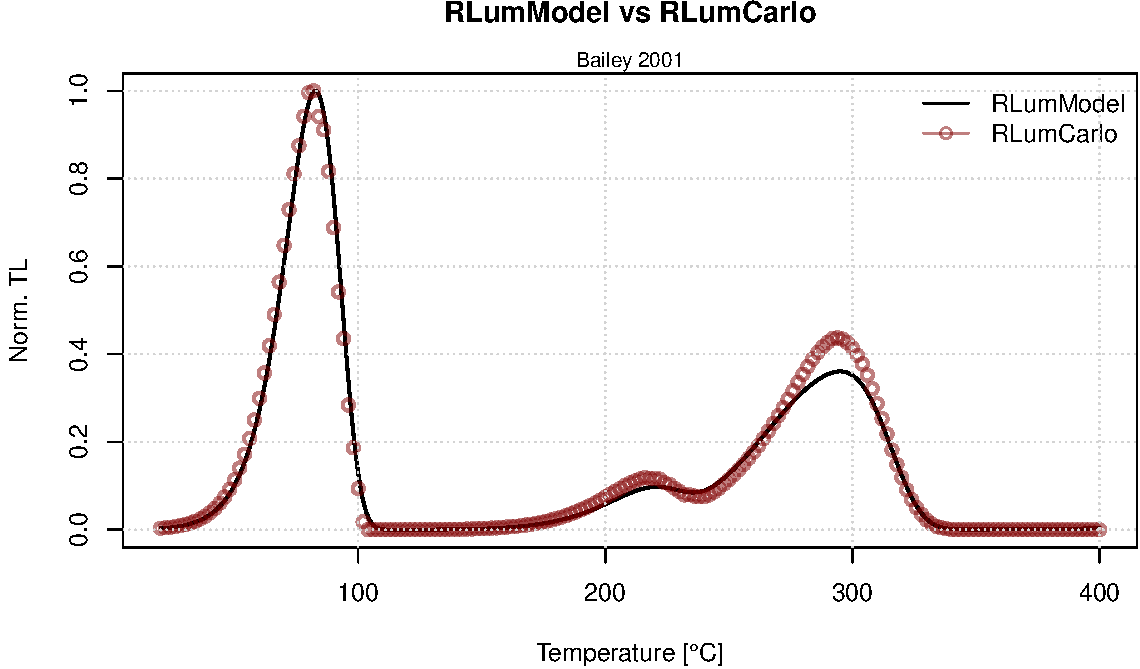
\includegraphics[width=90mm]{figures/Fig7-1} 

}

\caption[Simulation results of \CRANpkg{RLumModel} and \CRANpkg{RLumCarlo}]{Simulation results of \CRANpkg{RLumModel} and \CRANpkg{RLumCarlo}. Qualitatively both approaches show a good match.}\label{fig:Fig7}
\end{figure}
\end{Schunk}

\hypertarget{summary}{%
\section{Summary}\label{summary}}

The modeling of luminescence phenomena (cold light) of semiconductors
and insulators after having received ionizing radiation is a challenging
task. MC methods allow setting up flexible and simple systems to
simulate luminescence with a finite number of charge carriers. This
enables users to address effects usually observed for nano-dosimetric
systems, and it provides insight into the stochastic uncertainty
structure. We presented \CRANpkg{RLumCarlo}, which renders, to our best
knowledge, the first open-source and ready-to-use compilation of basic
MC luminescence models for different stimulation modes (so far CW-OSL,
LM-OSL, ISO-TL, and TL). We showed that the output from different models,
which are simulated in separate MC chains in virtual clusters, can be
combined to either simulate more complex systems or to mimic simple
spatial correlations between cluster groups. The way of the
implementation does not limit \CRANpkg{RLumCarlo} to a specific
dosimeter (e.g., quartz). In this light, \CRANpkg{RLumCarlo} can be used
in education, and research to test the impact of model
parameters, such as cluster sizes and related stochastic uncertainties.
Furthermore, \CRANpkg{RLumCarlo} can help in in formulating research
hypotheses and test them with commonly accepted or new models, still to
be developed.

Future work will implement more models to run as MC simulation, e.g.,
for irradiation processes in crystals (including its luminescence
output: radiofluorescence) and for an advanced interaction of clusters.

\hypertarget{acknowledgements}{%
\section{Acknowledgements}\label{acknowledgements}}

We thank two anonymous reviewers for their thorough reviews and
constructive suggestions, which helped to improve our manuscript.
Furthermore, we are grateful to the CRAN team in general for their
tireless efforts in keeping such a great resource alive and in
particular for their patience during the initial submission of
\CRANpkg{RLumCarlo}. Alex Roy Duncan is thanked for his support on the
package development during our stay in Westminster. The development of
\CRANpkg{RLumCarlo} benefited from the support of various funding
bodies. The initial work by JF, SK and CS was supported by the Deutsche
Forschungsgemeinschaft (2015--2018, DFG SCHM 3051/4-1, \emph{``Modelling
quartz luminescence signal dynamics relevant for dating and
dosimetry''}). Later financial support was secured through the project
\emph{``ULTIMO: Unifying Luminescence Models of quartz and feldspar''}
granted by the Deutscher Akademischer Austauschdienst (DAAD PPP USA
2018, ID: 57387041). SK was supported by the LabEx LaScArBx (ANR -
n.\(^{\circ}\)ANR-10-LABX-52) until 2019. From 2020, SK has received
funding from the European Union's Horizon 2020 research and innovation
program under the Marie Skłodowska-Curie grant agreement No 844457
(CREDit). This is IPGP contribution number 4202.

\bibliography{RLumCarlo_Manuscript}


\address{%
Sebastian Kreutzer\\
Department of Geography \& Earth Sciences, Aberystwyth University\\%
Aberystwyth\\ SY23 3DB, Wales, United Kingdom\\
IRAMAT-CRP2A, UMR 5060, CNRS-Université Bordeaux Montaigne\\%
Maison de l'Archéologie\\ Esplanade des Antilles\\ 36607 Pessac Cedex,
France\\
%
%
\\\textit{ORCiD: \href{https://orcid.org/0000-0001-9166-4563}{0000-0001-9166-4563}}%
\\\href{mailto:sebastian.kreutzer@aber.ac.uk}{\nolinkurl{sebastian.kreutzer@aber.ac.uk}}
}

\address{%
Johannes Friedrich\\
Chair of Geomorphology, University of Bayreuth\\%
Universitätsstr. 30\\ 95447 Bayreuth, Germany\\
%
%
\\\textit{ORCiD: \href{https://orcid.org/0000-0002-0805-9547}{0000-0002-0805-9547}}%
\\\href{mailto:johannes.friedrich@posteo.de}{\nolinkurl{johannes.friedrich@posteo.de}}
}

\address{%
Vasilis Pagonis\\
Physics Department, McDaniel College\\%
Westminster, MD 21157, USA\\
%
%
\\\textit{ORCiD: \href{https://orcid.org/0000-0002-4852-9312}{0000-0002-4852-9312}}%
\\\href{mailto:vpagonis@mcdaniel.edu}{\nolinkurl{vpagonis@mcdaniel.edu}}
}

\address{%
Christian Laag\\
Université de Paris, Institut de Physique du Globe de Paris, CNRS\\%
75005 Paris, France\\
Chair of Geomorphology, University of Bayreuth\\%
95447 Bayreuth, Germany\\
%
%
\\\textit{ORCiD: \href{https://orcid.org/0000-0002-6012-1029}{0000-0002-6012-1029}}%
\\\href{mailto:laag@ipgp.fr}{\nolinkurl{laag@ipgp.fr}}
}

\address{%
Ena Rajovic\\
Chair of Geomorphology, University of Bayreuth\\%
95447 Bayreuth, Germany\\
%
%
%
\\\href{mailto:ena.rajovic@uni-bayreuth.de}{\nolinkurl{ena.rajovic@uni-bayreuth.de}}
}

\address{%
Christoph Schmidt\\
Institute of Earth Surface Dynamics, University of Lausanne\\%
1015 Lausanne, Switzerland\\
%
%
\\\textit{ORCiD: \href{https://orcid.org/0000-0002-2309-3209}{0000-0002-2309-3209}}%
\\\href{mailto:christoph.schmidt@unil.ch}{\nolinkurl{christoph.schmidt@unil.ch}}
}
